\documentclass[pdf, aspectratio=169, 12pt]{beamer}
\usepackage[]{hyperref, graphicx, siunitx, lmodern, tikz, booktabs, physics}
\usepackage[mode=buildnew]{standalone}
\usepackage{pdfpc-commands}
\usepackage{pgfplots}
\pgfplotsset{compat=1.16}

\usetheme{Python}

\graphicspath{ {Images/} }

\sisetup{per-mode=symbol}
\usetikzlibrary{calc, patterns, decorations.markings, decorations.pathmorphing, shapes}

%Preamble
\title{File I/O: A Recurring Theme}
\author{Jed Rembold}
\date{February 26, 2020}

\begin{document}

\begin{frame}{Announcements}
	\begin{itemize}
		\item Homework
			\begin{itemize}
				\item Homework 5 is posted!
				\item No scanned work on this one, everything in the repository.
				\item I'm still working on grading HW4
			\end{itemize}
		\item Still working on grade reports, but now that my other tests are graded it may actually happen!
		\item Polling: \url{rembold-class.ddns.net}
	\end{itemize}
\end{frame}

\begin{frame}[fragile]{Review Question}
		We saw on Monday that the Fibonacci sequence can be written as a recursive function using the code to the right. Suppose you then wanted to know the 5th Fibonacci number, and thus called \pyi{fib(5)}. How many times does the \pyi{fib} function get called in total before the final value is returned to you?
	\begin{columns}
		\column{0.3\textwidth}
		\begin{poll}
		\item 1
		\item 4
		\item 6
		\item 9
		\end{poll}
		\exsol{9}
		\column{0.6\textwidth}
		\begin{pythoncode}[tabsize=2]
			def fib(n):
				if n == 1 or n == 2:
					return 1
				else:
					return fib(n-1) + fib(n-2)
		\end{pythoncode}
	\end{columns}
\end{frame}

\begin{frame}[fragile]{Not just for numbers}
	\begin{columns}
		\column{0.5\textwidth}
		\begin{itemize}
			\item Recursion is in no way restricted to numbers!
			\item Shows up graphically and visually
				\begin{itemize}
					\item Fractals for example
				\end{itemize}
			\item Can be useful in dealing with characters or strings as well
		\end{itemize}
		
		\column{0.5\textwidth}
		\begin{center}
			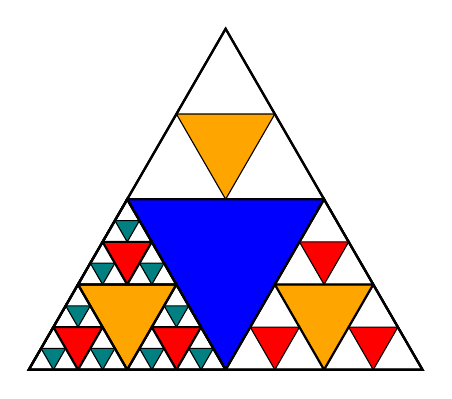
\begin{tikzpicture}
				\newcommand{\iter}[3]{
					\coordinate (A) at (#1);
					\coordinate (B) at ($(#1)+(60:#2)$);
					\coordinate (C) at ($(#1)+(0:#2)$);

					\coordinate (AB) at ($(A)!0.5!(B)$);
					\coordinate (AC) at ($(A)!0.5!(C)$);
					\coordinate (BC) at ($(B)!0.5!(C)$);

					\draw[thick] (A) -- (B) -- (C) -- cycle;
					\draw[fill=#3] (AB) -- (BC) -- (AC) -- cycle;
				}
				\newcommand{\grouptri}[3]{
					\iter{#1}{#2}{#3}
					\coordinate (p2) at ($(#1)+(60:#2)$);
					\iter{p2}{#2}{#3}
					\coordinate (p3) at ($(#1)+(0:#2)$);
					\iter{p3}{#2}{#3}
				}

				\newcommand{\serp}[1]{
					\iter{0,0}{#1}{Blue}

					\pgfmathsetmacro{\r}{#1/2}
					\grouptri{0,0}{\r}{Orange}

					\pgfmathsetmacro{\r}{\r/2}
					\grouptri{0,0}{\r}{Red}
					\grouptri{0:2*\r}{\r}{Red}
					%\grouptri{60:2*\r}{\r}{Red}

					\pgfmathsetmacro{\r}{\r/2}
					\grouptri{0,0}{\r}{Teal}
					\grouptri{0:2*\r}{\r}{Teal}
					\grouptri{60:2*\r}{\r}{Teal}
				}
				\serp{5}
			\end{tikzpicture}
		\end{center}
	\end{columns}
\end{frame}

\begin{frame}{Reversing a String}
	\begin{itemize}[<+->]
		\item Consider a general string:
			\begin{center}
				\pyi{"This is a great string"}
			\end{center}
		\item Could break it up and simplify the problem as:
			\begin{itemize}
				\item Move first character to the end
				\item Reverse the remaining of the characters
			\begin{center}
				\pyi{reverse("his is a great string") + "T"}
			\end{center}
			\end{itemize}
		\item What is the base case?
			\begin{itemize}
				\item Only a single letter left
				\item Return just that letter
			\end{itemize}
	\end{itemize}
\end{frame}

\begin{frame}{Pruning Duplicates}
	\begin{itemize}
		\item Consider the string:
			\begin{center}
				\pyi{"aabbccdeff"}
			\end{center}
		\item Want to return the string with no consecutive duplicates
		\item Base case:
			\begin{itemize}
				\item When a string length is 1
			\end{itemize}
		\item If first two values duplicates, skip one
		\item Otherwise store the first and run the function on the rest
	\end{itemize}
\end{frame}


\begin{frame}{Reading and Writing}
	\begin{itemize}
		\item<1-> Frequently want to save the result of some computation
			\begin{itemize}
				\item Maybe time intensive and do not want to run again
				\item Maybe need to manipulate results in a different program
				\item Maybe just need to store to view later
			\end{itemize}
		\item<2->Also need to be able to read in data from stored files
		\item<3-> Different operating systems have their own file systems
		\item<4-> Python uses \alert{file handles} to refer to an accessed file
			\begin{itemize}
				\item \pyi{name_of_handle = open('text.txt', 'w')}
			\end{itemize}
	\end{itemize}
\end{frame}

\begin{frame}[fragile]{The Flow of File I/O}
		\begin{itemize}
			\item Start by opening a file and giving it a handle
				\begin{itemize}
					\item Use appropriate option of \pyi{'w'}, \pyi{'r'}, or \pyi{'a'} depending on your use
				\end{itemize}
			\item Read or write lines or characters into file
				\begin{itemize}
					\item Frequently using loops, but to necessarily
				\end{itemize}
			\item Close the file!
		\end{itemize}
		\vspace{5mm}

		\begin{pythoncode}
			fhandle = open('Names.txt', 'w')
			for i in range(3):
				name = input('Enter a name: ')
				fhandle.write(name + '\n')
			fhandle.close()
		\end{pythoncode}
\end{frame}

\begin{frame}{Tis a New Line}
	\begin{itemize}
		\item Backslash is a special character in Python strings
		\item Signifies that the next character has special important
		\item \pyi{\n} signifies to the Python interpreter that a new line should start at that point.
		\item Can look invisible when printed but \emph{definitely} exist when comparing strings!
		\item Can always use \pyi{repr(some_string)} to see all the special characters
	\end{itemize}
\end{frame}

\begin{frame}{Reading from Files}
	\begin{itemize}
		\item Need the option \pyi{'r'} after the filename in \pyi{open}
		\item Python treats the file as a sequence of lines
			\begin{itemize}
				\item Can use \pyi{for} to iterate over all lines of the file
			\end{itemize}
		\item Be careful reading in lines to realize that you get all special characters as well!
			\begin{itemize}
				\item May want to use \pyi{.strip()} to remove trailing newline characters before comparisons
				\item Or index it out by including everything up to but not including the last character
			\end{itemize}
	\end{itemize}
\end{frame}


\begin{frame}{Intro to String Methods}
	\vspace{3mm}
	\begin{itemize}
		\item Python has a multitude of built-in string functions that you can use
		\item Accessed in a different manner than you are used to
			\begin{itemize}
				\item Use ``dot'' notation
				\item Technically \alert{methods}, a distinction which we'll talk more about later
				\item Can think of it as a function where the main argument comes first, then the function name and extra arguments
			\end{itemize}
		\item Examples:
			\begin{itemize}
				\item \pyi{'EXCITING'.lower()}
				\item \pyi{"excellent".count('e')}
			\end{itemize}
	\end{itemize}
	\pause
	\begin{alertblock}{Getting Help!}
		Curious about a potential string method you could use but don't know exactly what it does? Call the method but leave off the parentheses and add a \pyi{?} at the end!
	\end{alertblock}
\end{frame}















\end{document}

